\documentclass{article}
\usepackage[utf8]{inputenc}
\usepackage[margin=1in]{geometry}

\title{452 - Homework 2}
\author{Victor Zhang}
\date{February 3, 2020}

\usepackage[utf8]{inputenc}
\usepackage{amsmath}
\usepackage{amsfonts}
\usepackage{natbib}
\usepackage{graphicx}
% \usepackage{changepage}
\usepackage{amssymb}
\usepackage{xfrac}
% \usepackage{bm}
% \usepackage{empheq}
\usepackage{tikz}
\usetikzlibrary{arrows,automata}

\newcommand{\contra}{\raisebox{\depth}{\#}}

\newenvironment{myindentpar}[1]
  {\begin{list}{}
          {\setlength{\leftmargin}{#1}}
          \item[]
  }
  {\end{list}}

\pagestyle{empty}

\begin{document}

\maketitle
% \begin{center}
% {\huge Econ 482 \hspace{0.5cm} HW 3}\
% {\Large \textbf{Victor Zhang}}\
% {\Large February 18, 2020}
% \end{center}

\section*{1.4.e}
$A = \{w \;:\; w \text{ begins with } a\}$

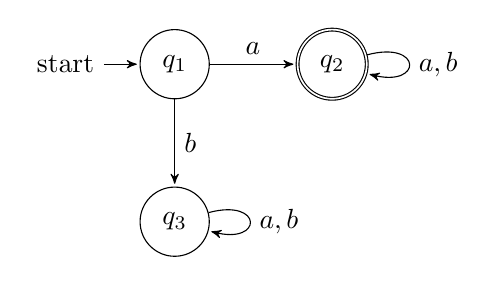
\begin{tikzpicture}[->,>=stealth',shorten >=1pt,auto,node distance=2cm,
        scale = 1,transform shape]

  \node[state,initial] (q_1) {$q_1$};
  \node[state,accepting] (q_2) [right of=q_1] {$q_2$};
  \node[state] (q_3) [below of=q_1] {$q_3$};

  \path (q_1) edge              node {$a$} (q_2)
        (q_1) edge              node {$b$} (q_3)
        (q_2) edge [loop right] node {$a,b$} (q_2)
        (q_3) edge [loop right] node {$a,b$} (q_3);

\end{tikzpicture}

\noindent
$B = \{w \;:\; w \text{ contains at most 1 } b\}$

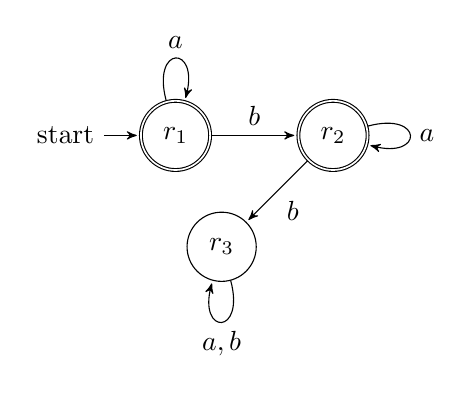
\begin{tikzpicture}[->,>=stealth',shorten >=1pt,auto,node distance=2cm,
        scale = 1,transform shape]

  \node[state,accepting,initial] (r_1) {$r_1$};
  \node[state,accepting] (r_2) [right of=r_1] {$r_2$};
  \node[state] (r_3) [below left of=r_2] {$r_3$};

  \path (r_1) edge [loop above] node {$a$} (r_1)
        (r_1) edge              node {$b$} (r_2)
        (r_2) edge [loop right] node {$a$} (r_2)
        (r_2) edge              node {$b$} (r_3)
        (r_3) edge [loop below] node {$a,b$} (r_3);

\end{tikzpicture}

\noindent
$A \cap B$

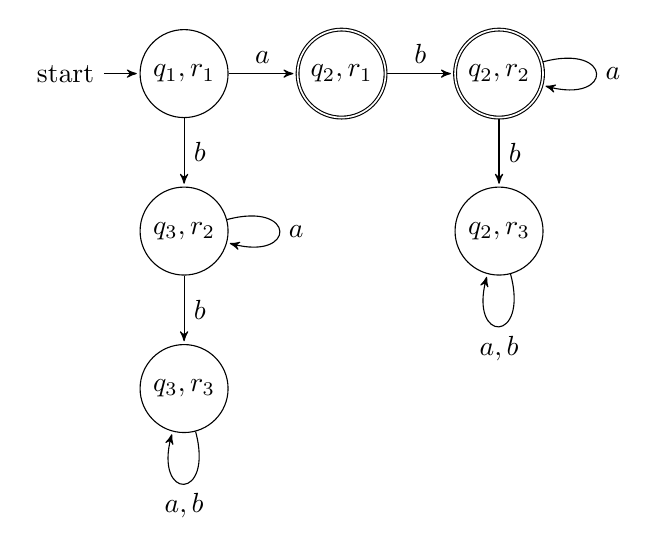
\begin{tikzpicture}[->,>=stealth',shorten >=1pt,auto,node distance=2cm,
        scale = 1,transform shape]

  \node[state,initial] (q_1r_1) {$q_1,r_1$};
  \node[state,accepting] (q_2r_1) [right of=q_1r_1] {$q_2,r_1$};
  \node[state] (q_3r_2) [below of=q_1r_1] {$q_3,r_2$};
  \node[state] (q_3r_3) [below of=q_3r_2] {$q_3,r_3$};
  \node[state,accepting] (q_2r_2) [right of=q_2r_1] {$q_2,r_2$};
  \node[state] (q_2r_3) [below of=q_2r_2] {$q_2,r_3$};

  \path (q_1r_1) edge              node {$a$} (q_2r_1)
        (q_1r_1) edge              node {$b$} (q_3r_2)
        (q_3r_2) edge [loop right] node {$a$} (q_3r_2)
        (q_3r_2) edge              node {$b$} (q_3r_3)
        (q_3r_3) edge [loop below] node {$a,b$} (q_3r_3)
        (q_2r_1) edge              node {$b$} (q_2r_2)
        (q_2r_2) edge [loop right] node {$a$} (q_2r_2)
        (q_2r_2) edge              node {$b$} (q_2r_3)
        (q_2r_3) edge [loop below] node {$a,b$} (q_2r_3);

\end{tikzpicture}

\section*{1.6.i}
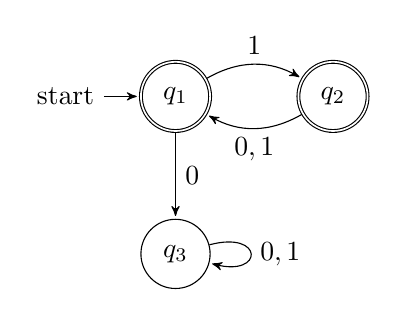
\begin{tikzpicture}[->,>=stealth',shorten >=1pt,auto,node distance=2cm,
        scale = 1,transform shape]

  \node[state,accepting,initial] (q_1) {$q_1$};
  \node[state,accepting] (q_2) [right of=q_1] {$q_2$};
  \node[state] (q_3) [below of=q_1] {$q_3$};

  \path (q_1) edge [bend left]  node {$1$} (q_2)
        (q_1) edge              node {$0$} (q_3)
        (q_3) edge [loop right] node {$0,1$} (q_3)
        (q_2) edge [bend left]  node {$0,1$} (q_1);

\end{tikzpicture}

\section*{1.6.l}
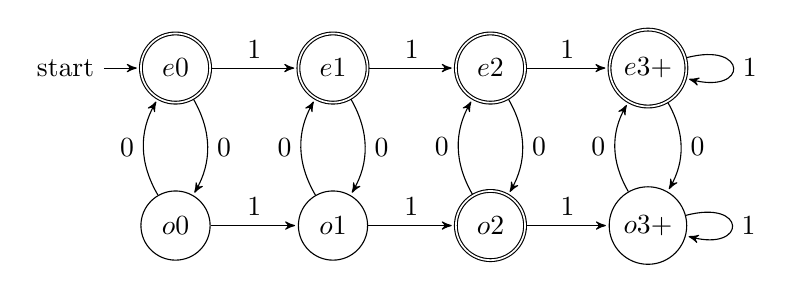
\begin{tikzpicture}[->,>=stealth',shorten >=1pt,auto,node distance=2cm,
        scale = 1,transform shape]

  \node[state,accepting,initial] (e0) {$e0$};
  \node[state] (o0) [below of=e0] {$o0$};
  \node[state,accepting] (e1) [right of=e0] {$e1$};
  \node[state] (o1) [below of=e1] {$o1$};
  \node[state,accepting] (e2) [right of=e1] {$e2$};
  \node[state,accepting] (o2) [below of=e2] {$o2$};
  \node[state,accepting] (e3+) [right of=e2] {$e3+$};
  \node[state] (o3+) [below of=e3+] {$o3+$};

  \path (e0) edge [bend left]  node {$0$} (o0)
        (o0) edge [bend left]  node {$0$} (e0)
        (e0) edge              node {$1$} (e1)
        (o0) edge              node {$1$} (o1)
        (e1) edge [bend left]  node {$0$} (o1)
        (o1) edge [bend left]  node {$0$} (e1)
        (e1) edge              node {$1$} (e2)
        (o1) edge              node {$1$} (o2)
        (e2) edge [bend left]  node {$0$} (o2)
        (o2) edge [bend left]  node {$0$} (e2)
        (e2) edge              node {$1$} (e3+)
        (o2) edge              node {$1$} (o3+)
        (e3+) edge [bend left]  node {$0$} (o3+)
        (o3+) edge [bend left]  node {$0$} (e3+)
        (e3+) edge [loop right] node {$1$} (e3+)
        (o3+) edge [loop right] node {$1$} (o3+);

\end{tikzpicture}

\section*{1.7.c}
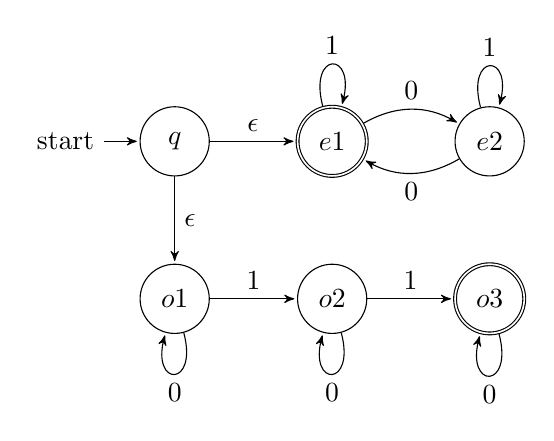
\begin{tikzpicture}[->,>=stealth',shorten >=1pt,auto,node distance=2cm,
        scale = 1,transform shape]

  \node[state,initial] (q) {$q$};
  \node[state,accepting] (e1) [right of=q] {$e1$};
  \node[state] (e2) [right of=e1] {$e2$};
  \node[state] (o1) [below of=q] {$o1$};
  \node[state] (o2) [right of=o1] {$o2$};
  \node[state,accepting] (o3) [right of=o2] {$o3$};

  \path (q) edge              node {$\epsilon$} (e1)
        (e1) edge [loop above] node {$1$} (e1)
        (e1) edge [bend left]  node {$0$} (e2)
        (e2) edge [bend left]  node {$0$} (e1)
        (e2) edge [loop above] node {$1$} (e2)
        (q) edge              node {$\epsilon$} (o1)
        (o1) edge [loop below] node {$0$} (o1)
        (o1) edge              node {$1$} (o2)
        (o2) edge [loop below] node {$0$} (o2)
        (o2) edge              node {$1$} (o3)
        (o3) edge [loop below] node {$0$} (o3);

\end{tikzpicture}

\section*{1.10.c}
The following state machine accepts the empty set.

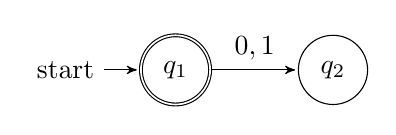
\begin{tikzpicture}[->,>=stealth',shorten >=1pt,auto,node distance=2cm,
        scale = 1,transform shape]

  \node[state,accepting,initial] (q_1) {$q_1$};
  \node[state] (q_2) [right of=q_1] {$q_2$};

  \path (q_1) edge              node {$0,1$} (q_2);

\end{tikzpicture}

\noindent
Following the proof of 1.49 we get the NFA

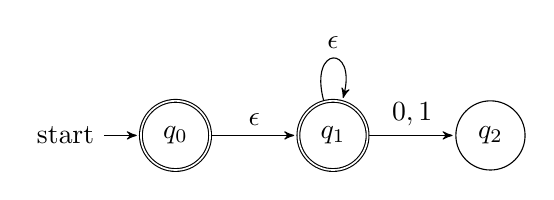
\begin{tikzpicture}[->,>=stealth',shorten >=1pt,auto,node distance=2cm,
        scale = 1,transform shape]

  \node[state,accepting] (q_1) {$q_1$};
  \node[state] (q_2) [right of=q_1] {$q_2$};
  \node[state,accepting,initial] (q_0) [left of=q_1] {$q_0$};

  \path (q_1) edge              node {$0,1$} (q_2)
        (q_1) edge [loop above] node {$\epsilon$} (q_1)
        (q_0) edge              node {$\epsilon$} (q_1);

\end{tikzpicture}

\noindent
which may be simplified to 

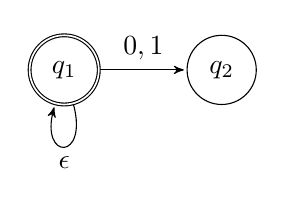
\begin{tikzpicture}[->,>=stealth',shorten >=1pt,auto,node distance=2cm,
        scale = 1,transform shape]

  \node[state,accepting] (q_1) {$q_1$};
  \node[state] (q_2) [right of=q_1] {$q_2$};

  \path (q_1) edge              node {$0,1$} (q_2)
        (q_1) edge [loop below] node {$\epsilon$} (q_1);

\end{tikzpicture}

\section*{1.14.b}
The below machine accepts $A = \{w \;:\; w \text{ ends with 1}\}$

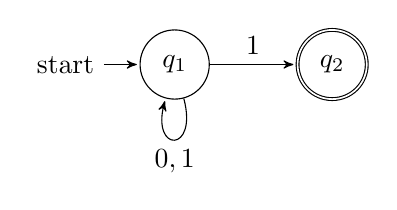
\begin{tikzpicture}[->,>=stealth',shorten >=1pt,auto,node distance=2cm,
        scale = 1,transform shape]

  \node[state,initial] (q_1) {$q_1$};
  \node[state,accepting] (q_2) [right of=q_1] {$q_2$};

  \path (q_1) edge [loop below] node {$0,1$} (q_1)
        (q_1) edge              node {$1$} (q_2);

\end{tikzpicture}

\noindent
However, the inverse does does not only accept $A^c = \{w \;:\; w \text{ does not end with 1}\}$. We may see that the machine accepts any string. Hence, NFAs are not closed to complement.

\section*{1.16.b}
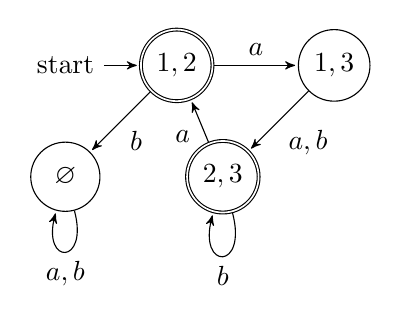
\begin{tikzpicture}[->,>=stealth',shorten >=1pt,auto,node distance=2cm,
        scale = 1,transform shape]

  \node[state,accepting,initial] (12) {$1,2$};
  \node[state] (13) [right of=12] {$1,3$};
  \node[state,accepting] (23) [below left of=13] {$2,3$};
  \node[state] (varempty) [below left of=12] {$\varnothing$};

  \path (12) edge              node {$a$} (13)
        (13) edge              node {$a,b$} (23)
        (23) edge [loop below] node {$b$} (23)
        (23) edge              node {$a$} (12)
        (12) edge              node {$b$} (varempty)
        (varempty) edge [loop below] node {$a,b$} (varempty);

\end{tikzpicture}

\section*{1.17.a}
First build an NFA that accepts the base language:

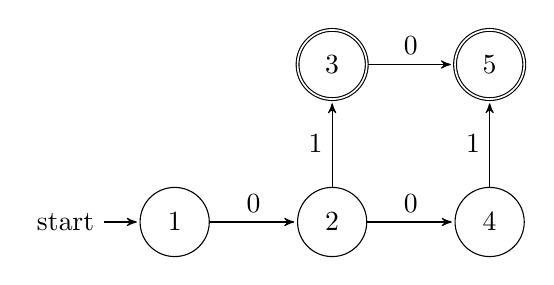
\begin{tikzpicture}[->,>=stealth',shorten >=1pt,auto,node distance=2cm,
        scale = 1,transform shape]

  \node[state,initial] (1) {$1$};
  \node[state] (2) [right of=1] {$2$};
  \node[state,accepting] (3) [above of=2] {$3$};
  \node[state] (4) [right of=2] {$4$};
  \node[state,accepting] (5) [above of=4] {$5$};

  \path (1) edge              node {$0$} (2)
        (2) edge              node {$1$} (3)
        (2) edge              node {$0$} (4)
        (3) edge              node {$0$} (5)
        (4) edge              node {$1$} (5);

\end{tikzpicture}

\noindent
Then construct an NFA accepting the Kleene star of this language:

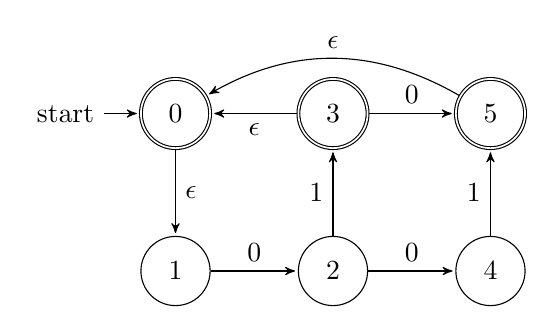
\begin{tikzpicture}[->,>=stealth',shorten >=1pt,auto,node distance=2cm,
        scale = 1,transform shape]

  \node[state,accepting,initial] (0) {$0$};
  \node[state] (1) [below of=0] {$1$};
  \node[state] (2) [right of=1] {$2$};
  \node[state,accepting] (3) [above of=2] {$3$};
  \node[state] (4) [right of=2] {$4$};
  \node[state,accepting] (5) [above of=4] {$5$};

  \path (1) edge              node {$0$} (2)
        (2) edge              node {$1$} (3)
        (2) edge              node {$0$} (4)
        (3) edge              node {$0$} (5)
        (4) edge              node {$1$} (5)
        (0) edge              node {$\epsilon$} (1)
        (3) edge              node {$\epsilon$} (0)
        (5) edge [bend right] node [above] {$\epsilon$} (0);

\end{tikzpicture}

\section*{1.17.b}
We write the power series expansion of the above NFA as

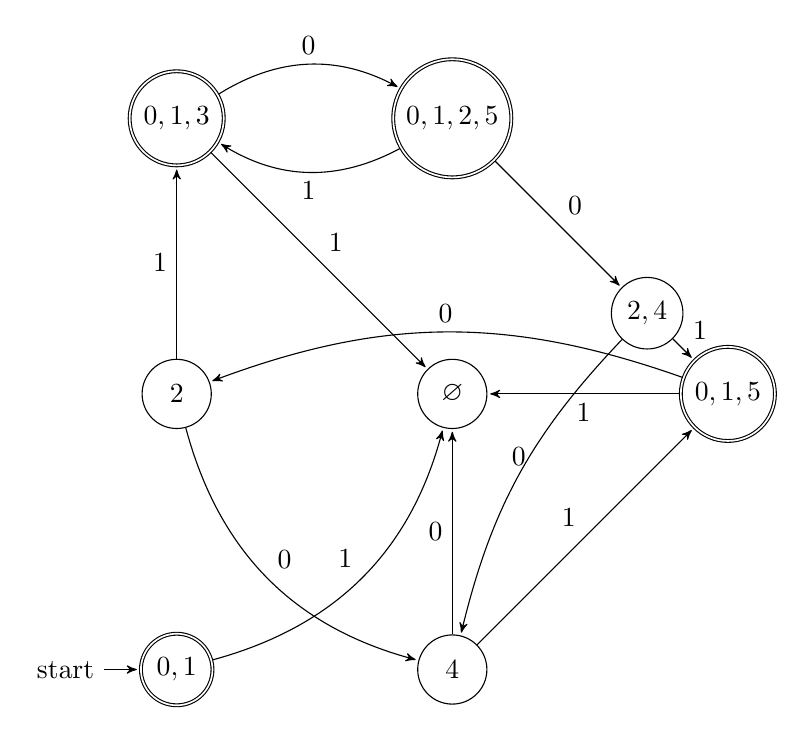
\begin{tikzpicture}[->,>=stealth',shorten >=1pt,auto,node distance=3.5cm,
        scale = 1,transform shape]

  \node[state,accepting,initial] (01) {$0,1$};
  \node[state] (2) [above of=01] {$2$};
  \node[state] (4) [right of=01] {$4$};
  \node[state] (empty) [right of=2] {$\varnothing$};
  \node[state,accepting] (013) [above of=2] {$0,1,3$};
  \node[state,accepting] (0125) [right of=013] {$0,1,2,5$};
  \node[state] (24) [below right of=0125] {$2,4$};
  \node[state,accepting] (015) [right of=empty] {$0,1,5$};

  \path (01) edge [bend right] node {$1$} (empty)
        (2) edge [bend right] node {$0$} (4)
        (2) edge              node {$1$} (013)
        (4) edge              node {$0$} (empty)
        (4) edge              node {$1$} (015)
        (015) edge              node {$1$} (empty)
        (015) edge [bend right=20] node [above] {$0$} (2)
        (013) edge              node {$1$} (empty)
        (013) edge [bend left]  node {$0$} (0125)
        (0125) edge [bend left]  node {$1$} (013)
        (0125) edge              node {$0$} (24)
        (24) edge [bend right=15] node [above] {$0$} (4)
        (24) edge              node {$1$} (015);

\end{tikzpicture}

\section*{1.18.i}
An accepted string may either have even or odd length. If it has odd length, the final character must be a 1. Otherwise, all odd positions should be 1 with no restriction on even positions:
$(1(0\cup1))^*(1\cup\epsilon)$

\section*{1.18.l}
We follow the procedure of replacing states and transitions with regular expressions. Starting with the original NFA

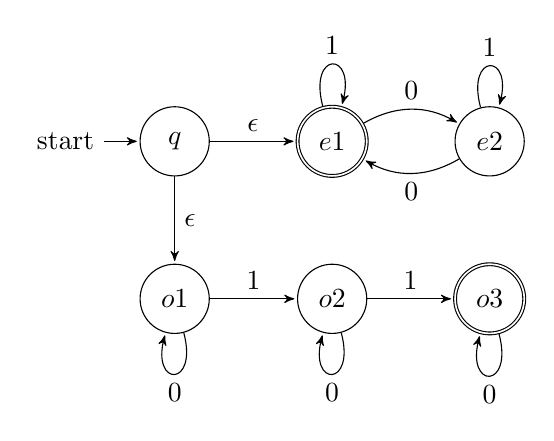
\begin{tikzpicture}[->,>=stealth',shorten >=1pt,auto,node distance=2cm,
        scale = 1,transform shape]

  \node[state,initial] (q) {$q$};
  \node[state,accepting] (e1) [right of=q] {$e1$};
  \node[state] (e2) [right of=e1] {$e2$};
  \node[state] (o1) [below of=q] {$o1$};
  \node[state] (o2) [right of=o1] {$o2$};
  \node[state,accepting] (o3) [right of=o2] {$o3$};

  \path (q) edge              node {$\epsilon$} (e1)
        (e1) edge [loop above] node {$1$} (e1)
        (e1) edge [bend left]  node {$0$} (e2)
        (e2) edge [bend left]  node {$0$} (e1)
        (e2) edge [loop above] node {$1$} (e2)
        (q) edge              node {$\epsilon$} (o1)
        (o1) edge [loop below] node {$0$} (o1)
        (o1) edge              node {$1$} (o2)
        (o2) edge [loop below] node {$0$} (o2)
        (o2) edge              node {$1$} (o3)
        (o3) edge [loop below] node {$0$} (o3);

\end{tikzpicture}

\noindent
We replace all the non-accepting states

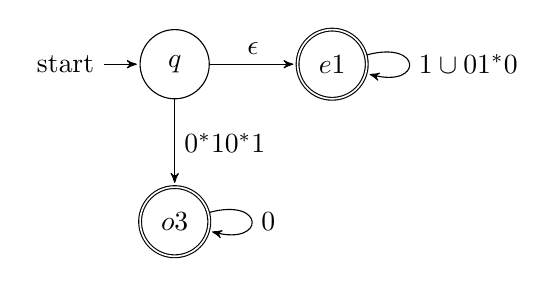
\begin{tikzpicture}[->,>=stealth',shorten >=1pt,auto,node distance=2cm,
        scale = 1,transform shape]

  \node[state,initial] (q) {$q$};
  \node[state,accepting] (e1) [right of=q] {$e1$};
  \node[state,accepting] (o3) [below of=q] {$o3$};

  \path (q) edge              node {$\epsilon$} (e1)
        (e1) edge [loop right] node {$1\cup01^*0$} (e1)
        (q) edge              node {$0^*10^*1$} (o3)
        (o3) edge [loop right] node {$0$} (o3);

\end{tikzpicture}

\noindent
The full regx is thus $(0^*10^*10^*)\cup(1\cup01^*0)^*$ $\Box$

\section*{1.31}
Let $M = (Q,\Sigma,\delta,q_0,F)$ be a DFA that accepts $A$. Generate a NFA $M' = (Q\cup{q'}, \Sigma, \delta',q,\{q'\})$ with a new accepting state $q'$, the transitions in $\delta$ reversed, transitions $\delta'(q,\epsilon) = r$ for all $r \in F$, and a transition $\delta'(q_0,\epsilon) = q$. We claim $M'$ accepts $A^\mathcal{R}$, so in fact $A^\mathcal{R}$ is regular. Indeed, suppose string $w \in A$ is accepted by $M$ through a sequence of states $q_0, \dots q_n$. Then $w^\mathcal{R}$ is accepted through the sequence $q,q_n,\dots q_0,q$. In addition, any $x \in A^\mathcal{R}$ that is accepted by $M'$ through some sequence $q,q_1,\dots q_n, q_0, q'$ may be mapped to an $x'$ which is accepted by sequence $q_0, q_n, \dots q_1$, since we are guaranteed that $q_1$ is an accepting state by the construction of $M'$ $\Box$

\section*{1.34}
The condition may be simplified to
$$\{w \;:\; \text{there is at least one occurrence of } \left[\begin{matrix}1\\0\end{matrix}\right] \text{ and there are no occurrences of } \left[\begin{matrix}0\\1\end{matrix}\right] \text{ before one of the former}\}$$
We may easily imagine a DFA which represents this condition, so $D$ is regular $\Box$

\section*{1.51}
Clearly, $\equiv_L$ is reflexive and symmetric. Now suppose $x\equiv_L y$ and $y \equiv_L w$. Then for all $z$, $xz \in L$ iff $yz \in L$, $yz \in L$ iff $wz \in L$. Thus $xz \in L$ iff $wz \in L$, so $x \equiv_L w$ and thus the relation is transitive and further an equivalence relation $\Box$

\end{document}

% List of tex snippets:
%   - tex-header (this)
%   - R      --> \mathbb{R}
%   - Z      --> \mathbb{Z}
%   - B      --> \mathcal{B}
%   - E      --> \mathcal{E}
%   - M      --> \mathcal{M}
%   - m      --> \mathfrak{m}({#1})
%   - normlp --> \norm{{#1}}_{L^{{#2}}}
